\chapter{Project Scheduling and Tracking}

\section{Work Breakdown Structure (WBS)}

Project scheduling is the project management discipline that organizes software engineering activities into manageable work packages, establishes temporal dependencies, assigns calendar durations, and identifies critical execution pathways.

The Work Breakdown Structure (WBS) decomposes the project hierarchically into four core operational levels:

\begin{lstlisting}
1.0 Bank Loan Management System
    1.1 Project Initiation & Requirement Engineering
        1.1.1 Stakeholder Interviews & Problem Identification
        1.1.2 Feasibility Study (Technical, Economic, Operational)
        1.1.3 Software Requirement Specification (SRS) Authoring
        1.1.4 Requirements Validation & Review Sign-off
    1.2 System Architecture & Design Modeling
        1.2.1 High-Level Architectural Design (3-Tier Topology)
        1.2.2 Structured Analysis (DFDs Level 0, 1, 2 & Structure Chart)
        1.2.3 Object-Oriented Analysis (Use Cases, Class, Object Diagrams)
        1.2.4 Dynamic Behavioral Modeling (State-Chart, Activity Diagrams)
        1.2.5 Interaction Modeling (Sequence & Collaboration Diagrams)
        1.2.6 Physical System Modeling (Component & Deployment Diagrams)
        1.2.7 Relational Database Schema Design & Normalization (3NF)
    1.3 Implementation Planning & Component Construction
        1.3.1 Database Schema Definition & Data Dictionary Construction
        1.3.2 Authentication & Role-Based Access Control Architecture
        1.3.3 Loan Application Ingestion Engine Design
        1.3.4 Document Storage & Verification Workflow Logic
        1.3.5 Mathematical EMI Amortization Algorithm Formulation
        1.3.6 Credit Scoring & Underwriting Rule Modeling
        1.3.7 Management Reporting & Audit Engine Design
    1.4 Software Quality Assurance & Verification
        1.4.1 Comprehensive Test Plan Formulation
        1.4.2 Black-Box & Boundary Value Test Case Specification
        1.4.3 Simulated Functional Test Execution & Verification
        1.4.4 Security, ACID Compliance & Integrity Review
    1.5 Project Management, Finalization & Submission
        1.5.1 Function Point Size & Effort Estimation
        1.5.2 CPM / PERT Schedule & Critical Path Determination
        1.5.3 Academic Project Documentation Compilation
        1.5.4 Final Faculty Review & Viva Voce Presentation
\end{lstlisting}

\section{Project Activities and Dependencies}

The project schedule spans a standardized 24-week (120 working days) academic semester timeline.

\subsection{Table 7.1: Project Activity Schedule}

\begin{table}[htbp]
\centering
\small
\resizebox{\textwidth}{!}{%
\begin{tabular}{l l l l l}
\toprule
\textbf{Activity ID} & \textbf{Activity Description} & \textbf{Immediate Predecessor} & \textbf{Duration (Working Days)} & \textbf{Responsible Role} \\
\midrule
\textbf{A1} & Problem Identification \& Scope Formulation & None & 5 & Project Analyst \\
\textbf{A2} & Feasibility Study Analysis & A1 & 5 & Systems Analyst \\
\textbf{A3} & Requirement Elicitation \& Analysis & A2 & 10 & Requirements Engineer \\
\textbf{A4} & SRS Document Authoring \& Baselining & A3 & 8 & Lead Systems Analyst \\
\textbf{A5} & System Architecture \& Tier Definition & A4 & 7 & Software Architect \\
\textbf{A6} & Structured Modeling (DFD L0/L1/L2, Structure Chart) & A5 & 8 & Systems Analyst \\
\textbf{A7} & Database Relational Design \& Normalization (3NF) & A5 & 9 & Database Designer \\
\textbf{A8} & Static UML Modeling (Use Case, Class, Object) & A6, A7 & 8 & UML Designer \\
\textbf{A9} & Dynamic UML Modeling (State-Chart, Activity) & A8 & 7 & UML Designer \\
\textbf{A10} & Interaction Modeling (Sequence, Collaboration) & A9 & 7 & UML Designer \\
\textbf{A11} & Physical UML Modeling (Component, Deployment) & A10 & 6 & Software Architect \\
\textbf{A12} & Core Business Algorithm Design (EMI, Scoring) & A7, A10 & 8 & Financial Systems Engineer \\
\textbf{A13} & Comprehensive Test Plan Formulation & A4, A11 & 6 & QA Lead \\
\textbf{A14} & Functional Test Case Design \& Black-Box Suites & A12, A13 & 9 & QA Test Engineer \\
\textbf{A15} & Simulated Test Execution \& Defect Reporting & A14 & 8 & QA Test Engineer \\
\textbf{A16} & Function Point Analysis (FPA) Estimation & A4, A11 & 6 & Project Manager \\
\textbf{A17} & Project Scheduling (PERT / CPM / Gantt) & A16 & 5 & Project Manager \\
\textbf{A18} & Project Risk Management \& SQA Planning & A17 & 4 & Project Manager \\
\textbf{A19} & Final Comprehensive Documentation \& Review & A15, A18 & 8 & Technical Writer / All \\
\bottomrule
\end{tabular}%
}
\end{table}

\section{Gantt Chart}

The Gantt Chart represents the temporal sequencing, concurrency, and milestone progressions of all 19 project work packages across the semester schedule.

\begin{figure}[htbp]
\centering
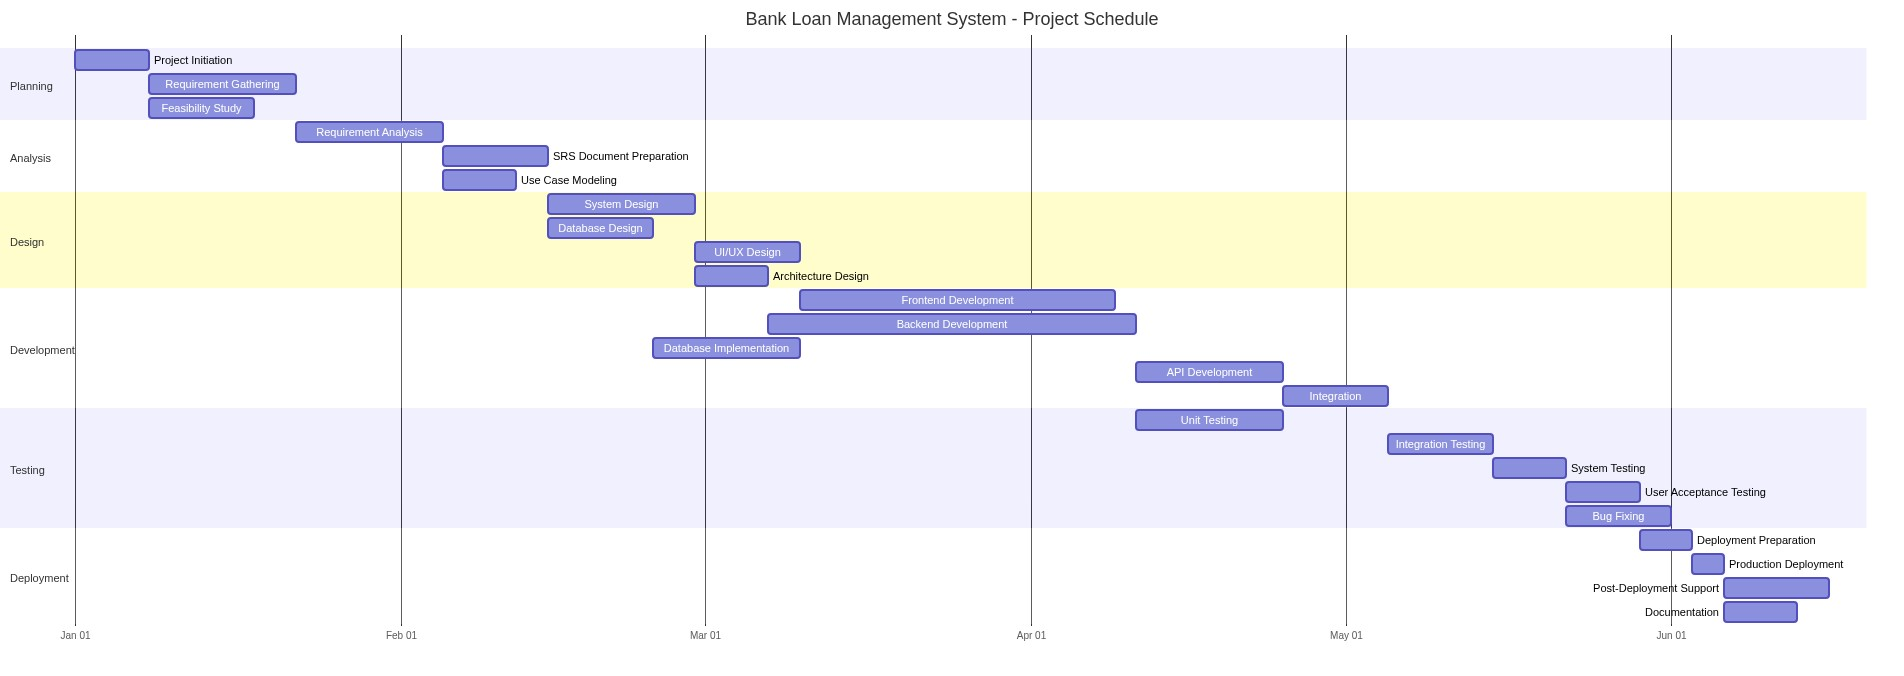
\includegraphics[width=0.85\textwidth]{figures/gantt_chart.png}
\caption{Figure 7.1: Project Schedule Gantt Chart}
\label{fig:gantt_chart}
\end{figure}

\textit{Figure 7.1: Project Schedule Gantt Chart}

\section{PERT Chart}

The Program Evaluation and Review Technique (PERT) Chart models the precedence network of the project as a directed graph, portraying concurrent activity paths, merge nodes, and dependency links.

\begin{figure}[htbp]
\centering
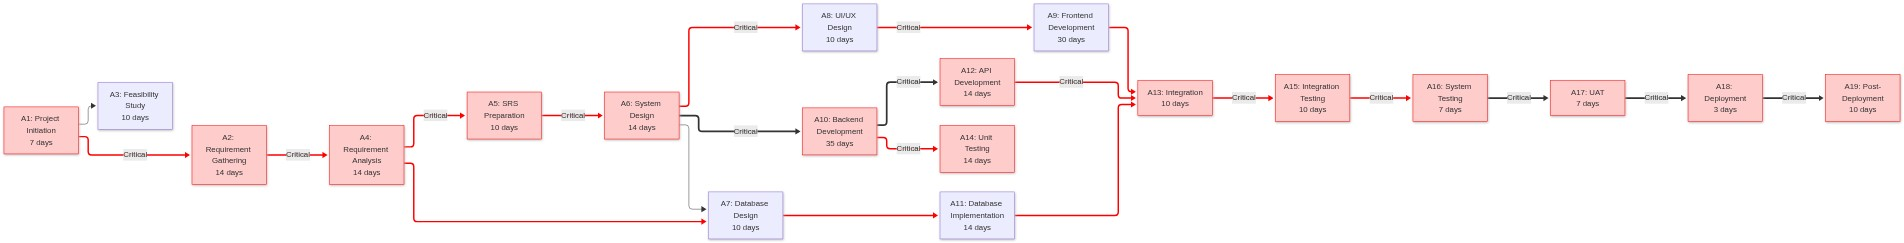
\includegraphics[width=0.85\textwidth]{figures/pert_chart.png}
\caption{Figure 7.2: PERT / CPM Network Diagram}
\label{fig:pert_chart}
\end{figure}

\textit{Figure 7.2: PERT / CPM Network Diagram}

\section{Critical Path Analysis (CPM)}

Critical Path Method (CPM) is a mathematical algorithm used for scheduling project activities. The Critical Path is the sequence of dependent activities that determines the minimum total calendar duration of the project. Any delay in an activity lying on the critical path results in an immediate day-for-day delay of the entire project completion date.

\subsection{Forward Pass (Early Start and Early Finish Calculation)}

\begin{itemize}
  \item \_\_INLINE\_MATH\_0\_\_: The earliest possible time an activity can commence:
\end{itemize}

\_\_DISPLAY\_MATH\_0\_\_

\begin{itemize}
  \item \_\_INLINE\_MATH\_0\_\_: The earliest possible time an activity can conclude:
\end{itemize}

\_\_DISPLAY\_MATH\_0\_\_

\subsection{Backward Pass (Late Start and Late Finish Calculation)}

\begin{itemize}
  \item \_\_INLINE\_MATH\_0\_\_: The latest possible time an activity can conclude without delaying project completion:
\end{itemize}

\_\_DISPLAY\_MATH\_0\_\_

\begin{itemize}
  \item \_\_INLINE\_MATH\_0\_\_: The latest possible time an activity can commence without delaying project completion:
\end{itemize}

\_\_DISPLAY\_MATH\_0\_\_

\subsection{Total Float (Slack Time) Calculation}

\begin{itemize}
  \item \_\_INLINE\_MATH\_0\_\_
  \item An activity is \textbf{Critical} if and only if \_\_INLINE\_MATH\_0\_\_.
\end{itemize}

\subsection{Table 7.2: Critical Path Mathematical Computation Table}

\begin{table}[htbp]
\centering
\small
\resizebox{\textwidth}{!}{%
\begin{tabular}{l l l l l l l l l}
\toprule
\textbf{Activity ID} & \textbf{Duration (\_\_MATH\_0\_\_)} & \textbf{Predecessors} & \textbf{Early Start (ES)} & \textbf{Early Finish (EF)} & \textbf{Late Start (LS)} & \textbf{Late Finish (LF)} & \textbf{Total Float (Slack)} & \textbf{Critical?} \\
\midrule
\textbf{A1} & 5 & None & 0 & 5 & 0 & 5 & 0 & \textbf{YES (Critical)} \\
\textbf{A2} & 5 & A1 & 5 & 10 & 5 & 10 & 0 & \textbf{YES (Critical)} \\
\textbf{A3} & 10 & A2 & 10 & 20 & 10 & 20 & 0 & \textbf{YES (Critical)} \\
\textbf{A4} & 8 & A3 & 20 & 28 & 20 & 28 & 0 & \textbf{YES (Critical)} \\
\textbf{A5} & 7 & A4 & 28 & 35 & 28 & 35 & 0 & \textbf{YES (Critical)} \\
\textbf{A6} & 8 & A5 & 35 & 43 & 36 & 44 & 1 & No \\
\textbf{A7} & 9 & A5 & 35 & 44 & 35 & 44 & 0 & \textbf{YES (Critical)} \\
\textbf{A8} & 8 & A6, A7 & 44 & 52 & 44 & 52 & 0 & \textbf{YES (Critical)} \\
\textbf{A9} & 7 & A8 & 52 & 59 & 52 & 59 & 0 & \textbf{YES (Critical)} \\
\textbf{A10} & 7 & A9 & 59 & 66 & 59 & 66 & 0 & \textbf{YES (Critical)} \\
\textbf{A11} & 6 & A10 & 66 & 72 & 68 & 74 & 2 & No \\
\textbf{A12} & 8 & A7, A10 & 66 & 74 & 66 & 74 & 0 & \textbf{YES (Critical)} \\
\textbf{A13} & 6 & A4, A11 & 72 & 78 & 74 & 80 & 2 & No \\
\textbf{A14} & 9 & A12, A13 & 74 & 83 & 74 & 83 & 0 & \textbf{YES (Critical)} \\
\textbf{A15} & 8 & A14 & 83 & 91 & 83 & 91 & 0 & \textbf{YES (Critical)} \\
\textbf{A16} & 6 & A4, A11 & 72 & 78 & 78 & 84 & 6 & No \\
\textbf{A17} & 5 & A16 & 78 & 83 & 84 & 89 & 6 & No \\
\textbf{A18} & 4 & A17 & 83 & 87 & 89 & 93 & 6 & No \\
\textbf{A19} & 8 & A15, A18 & 91 & 99 & 91 & 99 & 0 & \textbf{YES (Critical)} \\
\bottomrule
\end{tabular}%
}
\end{table}

\subsection{Identified Critical Path}

\_\_INLINE\_MATH\_0\_\_\textbackslash{}mathbf{	ext{Critical Path}} = \textbackslash{}mathbf{A1

ightarrow A2

ightarrow A3

ightarrow A4

ightarrow A5

ightarrow A7

ightarrow A8

ightarrow A9

ightarrow A10

ightarrow A12

ightarrow A14

ightarrow A15

ightarrow A19}\_\_INLINE\_MATH\_0\_\_

\begin{itemize}
  \item \textbf{Total Critical Duration:} \_\_INLINE\_MATH\_0\_\_ (approx. 20 calendar weeks).
  \item \textbf{Project Buffer:} The remaining 21 working days out of the 120-day semester schedule serve as an operational safety buffer accommodating review cycles, documentation polishing, and academic defense preparation.
\end{itemize}
